\documentclass[]{article}
\usepackage{lmodern}
\usepackage{amssymb,amsmath}
\usepackage{ifxetex,ifluatex}
\usepackage{fixltx2e} % provides \textsubscript
\ifnum 0\ifxetex 1\fi\ifluatex 1\fi=0 % if pdftex
  \usepackage[T1]{fontenc}
  \usepackage[utf8]{inputenc}
\else % if luatex or xelatex
  \ifxetex
    \usepackage{mathspec}
  \else
    \usepackage{fontspec}
  \fi
  \defaultfontfeatures{Ligatures=TeX,Scale=MatchLowercase}
\fi
% use upquote if available, for straight quotes in verbatim environments
\IfFileExists{upquote.sty}{\usepackage{upquote}}{}
% use microtype if available
\IfFileExists{microtype.sty}{%
\usepackage{microtype}
\UseMicrotypeSet[protrusion]{basicmath} % disable protrusion for tt fonts
}{}
\usepackage[margin=1in]{geometry}
\usepackage{hyperref}
\hypersetup{unicode=true,
            pdftitle={Model Parameter Inference \& Model Selection},
            pdfauthor={Robert Edwards},
            pdfborder={0 0 0},
            breaklinks=true}
\urlstyle{same}  % don't use monospace font for urls
\usepackage{color}
\usepackage{fancyvrb}
\newcommand{\VerbBar}{|}
\newcommand{\VERB}{\Verb[commandchars=\\\{\}]}
\DefineVerbatimEnvironment{Highlighting}{Verbatim}{commandchars=\\\{\}}
% Add ',fontsize=\small' for more characters per line
\usepackage{framed}
\definecolor{shadecolor}{RGB}{248,248,248}
\newenvironment{Shaded}{\begin{snugshade}}{\end{snugshade}}
\newcommand{\KeywordTok}[1]{\textcolor[rgb]{0.13,0.29,0.53}{\textbf{#1}}}
\newcommand{\DataTypeTok}[1]{\textcolor[rgb]{0.13,0.29,0.53}{#1}}
\newcommand{\DecValTok}[1]{\textcolor[rgb]{0.00,0.00,0.81}{#1}}
\newcommand{\BaseNTok}[1]{\textcolor[rgb]{0.00,0.00,0.81}{#1}}
\newcommand{\FloatTok}[1]{\textcolor[rgb]{0.00,0.00,0.81}{#1}}
\newcommand{\ConstantTok}[1]{\textcolor[rgb]{0.00,0.00,0.00}{#1}}
\newcommand{\CharTok}[1]{\textcolor[rgb]{0.31,0.60,0.02}{#1}}
\newcommand{\SpecialCharTok}[1]{\textcolor[rgb]{0.00,0.00,0.00}{#1}}
\newcommand{\StringTok}[1]{\textcolor[rgb]{0.31,0.60,0.02}{#1}}
\newcommand{\VerbatimStringTok}[1]{\textcolor[rgb]{0.31,0.60,0.02}{#1}}
\newcommand{\SpecialStringTok}[1]{\textcolor[rgb]{0.31,0.60,0.02}{#1}}
\newcommand{\ImportTok}[1]{#1}
\newcommand{\CommentTok}[1]{\textcolor[rgb]{0.56,0.35,0.01}{\textit{#1}}}
\newcommand{\DocumentationTok}[1]{\textcolor[rgb]{0.56,0.35,0.01}{\textbf{\textit{#1}}}}
\newcommand{\AnnotationTok}[1]{\textcolor[rgb]{0.56,0.35,0.01}{\textbf{\textit{#1}}}}
\newcommand{\CommentVarTok}[1]{\textcolor[rgb]{0.56,0.35,0.01}{\textbf{\textit{#1}}}}
\newcommand{\OtherTok}[1]{\textcolor[rgb]{0.56,0.35,0.01}{#1}}
\newcommand{\FunctionTok}[1]{\textcolor[rgb]{0.00,0.00,0.00}{#1}}
\newcommand{\VariableTok}[1]{\textcolor[rgb]{0.00,0.00,0.00}{#1}}
\newcommand{\ControlFlowTok}[1]{\textcolor[rgb]{0.13,0.29,0.53}{\textbf{#1}}}
\newcommand{\OperatorTok}[1]{\textcolor[rgb]{0.81,0.36,0.00}{\textbf{#1}}}
\newcommand{\BuiltInTok}[1]{#1}
\newcommand{\ExtensionTok}[1]{#1}
\newcommand{\PreprocessorTok}[1]{\textcolor[rgb]{0.56,0.35,0.01}{\textit{#1}}}
\newcommand{\AttributeTok}[1]{\textcolor[rgb]{0.77,0.63,0.00}{#1}}
\newcommand{\RegionMarkerTok}[1]{#1}
\newcommand{\InformationTok}[1]{\textcolor[rgb]{0.56,0.35,0.01}{\textbf{\textit{#1}}}}
\newcommand{\WarningTok}[1]{\textcolor[rgb]{0.56,0.35,0.01}{\textbf{\textit{#1}}}}
\newcommand{\AlertTok}[1]{\textcolor[rgb]{0.94,0.16,0.16}{#1}}
\newcommand{\ErrorTok}[1]{\textcolor[rgb]{0.64,0.00,0.00}{\textbf{#1}}}
\newcommand{\NormalTok}[1]{#1}
\usepackage{longtable,booktabs}
\usepackage{graphicx,grffile}
\makeatletter
\def\maxwidth{\ifdim\Gin@nat@width>\linewidth\linewidth\else\Gin@nat@width\fi}
\def\maxheight{\ifdim\Gin@nat@height>\textheight\textheight\else\Gin@nat@height\fi}
\makeatother
% Scale images if necessary, so that they will not overflow the page
% margins by default, and it is still possible to overwrite the defaults
% using explicit options in \includegraphics[width, height, ...]{}
\setkeys{Gin}{width=\maxwidth,height=\maxheight,keepaspectratio}
\IfFileExists{parskip.sty}{%
\usepackage{parskip}
}{% else
\setlength{\parindent}{0pt}
\setlength{\parskip}{6pt plus 2pt minus 1pt}
}
\setlength{\emergencystretch}{3em}  % prevent overfull lines
\providecommand{\tightlist}{%
  \setlength{\itemsep}{0pt}\setlength{\parskip}{0pt}}
\setcounter{secnumdepth}{5}
% Redefines (sub)paragraphs to behave more like sections
\ifx\paragraph\undefined\else
\let\oldparagraph\paragraph
\renewcommand{\paragraph}[1]{\oldparagraph{#1}\mbox{}}
\fi
\ifx\subparagraph\undefined\else
\let\oldsubparagraph\subparagraph
\renewcommand{\subparagraph}[1]{\oldsubparagraph{#1}\mbox{}}
\fi

%%% Use protect on footnotes to avoid problems with footnotes in titles
\let\rmarkdownfootnote\footnote%
\def\footnote{\protect\rmarkdownfootnote}

%%% Change title format to be more compact
\usepackage{titling}

% Create subtitle command for use in maketitle
\newcommand{\subtitle}[1]{
  \posttitle{
    \begin{center}\large#1\end{center}
    }
}

\setlength{\droptitle}{-2em}
  \title{Model Parameter Inference \& Model Selection}
  \pretitle{\vspace{\droptitle}\centering\huge}
  \posttitle{\par}
  \author{Robert Edwards}
  \preauthor{\centering\large\emph}
  \postauthor{\par}
  \predate{\centering\large\emph}
  \postdate{\par}
  \date{2/28/2019}

\usepackage{booktabs}
\usepackage{longtable}
\usepackage{array}
\usepackage{multirow}
\usepackage[table]{xcolor}
\usepackage{wrapfig}
\usepackage{float}
\usepackage{colortbl}
\usepackage{pdflscape}
\usepackage{tabu}
\usepackage{threeparttable}
\usepackage[normalem]{ulem}

\usepackage{float} \floatplacement{figure}{H}

\begin{document}
\maketitle

\section{Introduction}\label{sec:Intro}

In week 7 lab we considered the construction and use of confidence
intervals (CIs) for the population parameters listed in Table 1. In
particular, we used bootstrap methods to estimate the sampling
distributions of the estimates in Scenarios 1-4 and used these to
contruct CIs for the corresponding population parameters.

\begin{longtable}[]{@{}lcrrc@{}}
\toprule
Scenario & Population parameter & Population Notation & Point
estimate/sample statistic & Sample Notation\tabularnewline
\midrule
\endhead
1 & Population proportion & \(p\) & Sample proportion &
\(\hat{p}\)\tabularnewline
2 & Population mean & \(\mu\) & Sample mean & \(\bar{x}\)\tabularnewline
3 & Difference in population proportions & \(p_1-p_2\) & Difference in
sample proporti & ons \(\hat{p}_1-\hat{p}_2\)\tabularnewline
4 & Difference in population means & \(\mu_1-\mu_2\) & Difference in
sample means & \(\bar{x}_1-\bar{x}_2\)\tabularnewline
5 & Population regression intercept & \(\beta_0\) & Sample regression
intercept & \(\hat{\beta}_0~or~b_0\)\tabularnewline
6 & Population regression slope & \(\beta_1\) & Sample regression slope
& \(\hat{\beta}_1~or~b_1\)\tabularnewline
\bottomrule
\end{longtable}

In this week's lab we will continue this process for Scenarios 5 and 6,
namely construct CIs for the parameters in simple and multiple linear
regression models. We will start with bootstrap methods and also
consider CIs based on theoretical results when standard assumptions
hold. We will also consider how to use CIs for variable selection and
finish by considering a model selection strategy based on objective
measures for model comparisons.

\newpage

\section{Confidence Intervals for Regression
Parameters}\label{sec:regression}

\subsection{\texorpdfstring{Bootstrap Confidence Intervals for \(\beta\)
in Simple Linear Regression
(SLR)}{Bootstrap Confidence Intervals for \textbackslash{}beta in Simple Linear Regression (SLR)}}\label{bootstrap-confidence-intervals-for-beta-in-simple-linear-regression-slr}

Just as we did for Scenarios 1-4 in Table 1 in Week 7, we can use the
\texttt{infer} package to repeatedly sample from a dataset to estimate
the sampling distribution and standard error of the estimates of the
intercept (\(\hat{\alpha}\)) and the covariate's parameter
(\(\hat{\beta}\)) in the simple linear regression model
\(\hat{y} = \hat{\alpha} + \hat{\beta}x_i\). These sampling
distributions enable us to directly find bootstrap confidence intervals
for the model parameters. Usually, interest lies in \(\beta\) and so
that will be our focus here.

To illustrate this, let's return to the teaching evaluations data that
we analyzed last week and start with the SLR model with \texttt{age} as
the the single explanatory variable and the instructors' evaluation
\texttt{score}s as the outcome variable. This data and the fitted model
are shown here.

\begin{Shaded}
\begin{Highlighting}[]
\NormalTok{slr.model <-}\StringTok{ }\KeywordTok{lm}\NormalTok{(score}\OperatorTok{~}\NormalTok{age, }\DataTypeTok{data=}\NormalTok{evals)}
\NormalTok{coeff <-}\StringTok{ }\NormalTok{slr.model }\OperatorTok\StringTok{ }\KeywordTok{coef}\NormalTok{()}
\NormalTok{coeff}
\end{Highlighting}
\end{Shaded}

\begin{verbatim}
 (Intercept)          age 
 4.461932354 -0.005938225 
\end{verbatim}

\begin{Shaded}
\begin{Highlighting}[]
\KeywordTok{ggplot}\NormalTok{(evals, }\KeywordTok{aes}\NormalTok{(}\DataTypeTok{x =}\NormalTok{ age, }\DataTypeTok{y =}\NormalTok{ score)) }\OperatorTok{+}\StringTok{ }
\StringTok{  }\KeywordTok{geom_jitter}\NormalTok{() }\OperatorTok{+}
\StringTok{  }\KeywordTok{labs}\NormalTok{(}\DataTypeTok{x =} \StringTok{"Age"}\NormalTok{, }\DataTypeTok{y=} \StringTok{"Teaching Score"}\NormalTok{) }\OperatorTok{+}
\StringTok{  }\KeywordTok{geom_smooth}\NormalTok{(}\DataTypeTok{method =} \StringTok{"lm"}\NormalTok{, }\DataTypeTok{se =} \OtherTok{FALSE}\NormalTok{)}
\end{Highlighting}
\end{Shaded}

\begin{figure}
\centering
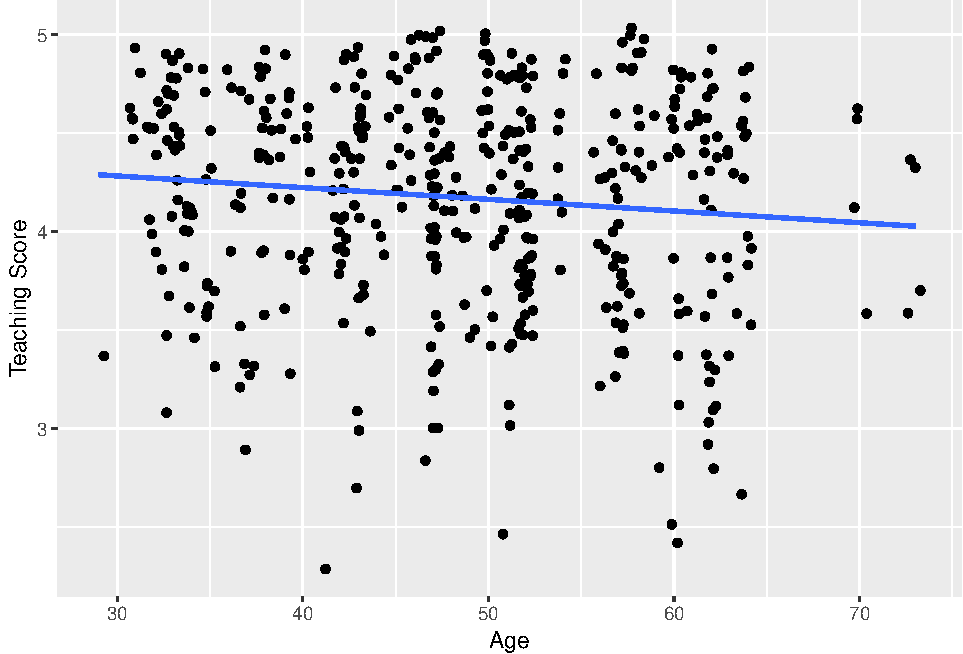
\includegraphics{DAWeek8_files/figure-latex/slr.model-1.pdf}
\caption{\label{fig.plot1}SLR Model applied to Teaching Evaluation Data}
\end{figure}

The point estimate of the slope parameter here is
\(\hat{\beta} = -0.006\). The following code estimates the sampling
distribution of \(\hat{\beta}\) via the bootstrap method.

\begin{Shaded}
\begin{Highlighting}[]
\NormalTok{bootstrap_beta_distn <-}\StringTok{ }\NormalTok{evals }\OperatorTok
\StringTok{  }\KeywordTok{specify}\NormalTok{(score }\OperatorTok{~}\StringTok{ }\NormalTok{age) }\OperatorTok
\StringTok{  }\KeywordTok{generate}\NormalTok{(}\DataTypeTok{reps =} \DecValTok{1000}\NormalTok{, }\DataTypeTok{type =} \StringTok{"bootstrap"}\NormalTok{) }\OperatorTok
\StringTok{  }\KeywordTok{calculate}\NormalTok{(}\DataTypeTok{stat =} \StringTok{"slope"}\NormalTok{)}

\NormalTok{bootstrap_beta_distn }\OperatorTok\StringTok{ }\KeywordTok{visualize}\NormalTok{()}
\end{Highlighting}
\end{Shaded}

\begin{figure}
\centering
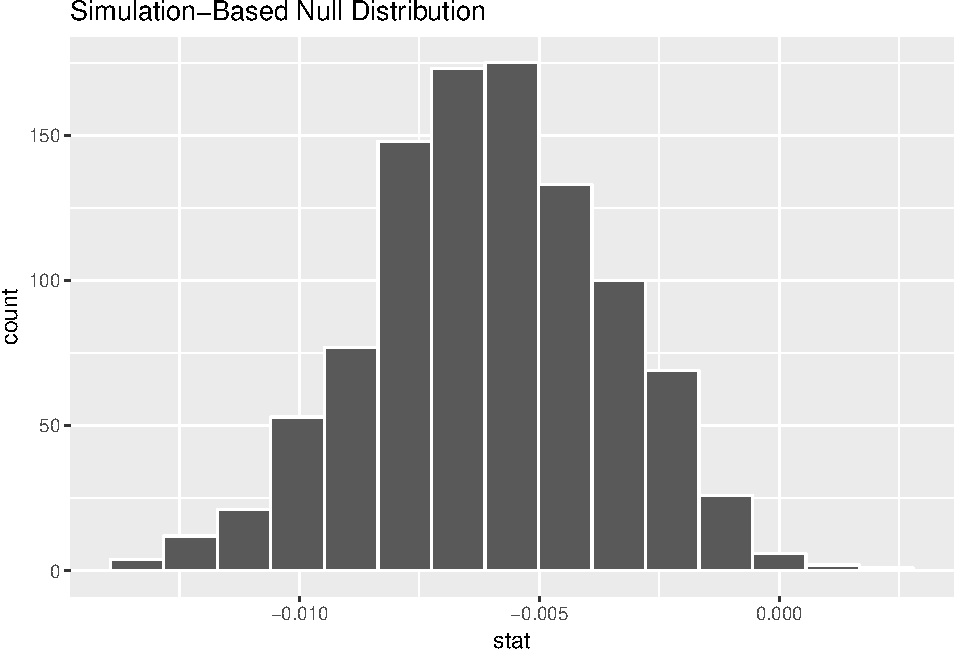
\includegraphics{DAWeek8_files/figure-latex/sampling1-1.pdf}
\caption{\label{fig.sampling1}Estimated distribution of parameters via
the bootstrap method}
\end{figure}

Now we can use the \texttt{get\_ci()} function to calculate a 95\%
confidence interval and a 99\% confidence interval. We can do this
either using the percentiles of the bootstrap distribution or using an
estimate of the standard error from the bootstrap distribution. Remember
that both these CIs denote a range of plausible values for the unknown
true population slope parameter regressing teaching \texttt{score} on
\texttt{age}.

\begin{Shaded}
\begin{Highlighting}[]
\NormalTok{percentile_beta_ci <-}\StringTok{ }\NormalTok{bootstrap_beta_distn }\OperatorTok
\StringTok{  }\KeywordTok{get_ci}\NormalTok{(}\DataTypeTok{level =} \FloatTok{0.95}\NormalTok{, }\DataTypeTok{type =} \StringTok{"percentile"}\NormalTok{)}
\NormalTok{percentile_beta_ci}
\end{Highlighting}
\end{Shaded}

\begin{verbatim}
# A tibble: 1 x 2
   `2.5%`   `97.5%`
    <dbl>     <dbl>
1 -0.0109 -0.000887
\end{verbatim}

\begin{Shaded}
\begin{Highlighting}[]
\NormalTok{se_beta_ci <-}\StringTok{ }\NormalTok{bootstrap_beta_distn }\OperatorTok
\StringTok{  }\KeywordTok{get_ci}\NormalTok{(}\DataTypeTok{level =} \FloatTok{0.99}\NormalTok{, }\DataTypeTok{type =} \StringTok{"se"}\NormalTok{, }\DataTypeTok{point_estimate =}\NormalTok{ coeff[}\DecValTok{2}\NormalTok{])}
\NormalTok{se_beta_ci}
\end{Highlighting}
\end{Shaded}

\begin{verbatim}
# A tibble: 1 x 2
    lower    upper
    <dbl>    <dbl>
1 -0.0125 0.000649
\end{verbatim}

\textbf{What is the 95\% confidence interval of the simulated bootstrap
sampling distribution using the 2.5\% and the 97.5\% percentiles?}

\begin{itemize}
\tightlist
\item
  (-0.011, -0.001)
\end{itemize}

\textbf{What is the 99\% confidence interval for the age parameter by
the standard error approach?}

\begin{itemize}
\tightlist
\item
  (-0.013, 0.001)
\end{itemize}

\textbf{Comparing the two different confidence intervals (95\% and 99\%)
produced by the \texttt{percentile} and the \texttt{se} methods,
respectively, we conclude:}

\begin{itemize}
\tightlist
\item
  \emph{The two confidence intervals are similar since the bootstrap
  sampling distribution was close to symmetric}
\end{itemize}

\subsection{Confidence Intervals for the Parameters in Multiple
Regression}\label{confidence-intervals-for-the-parameters-in-multiple-regression}

Let's continue with the teaching evaluations data by fitting the
multiple regression with one numerical and one categorical predictor
that we first saw in Week 6. In this model:

\begin{itemize}
\tightlist
\item
  \(y\): outcome variable of instructor evaluation \texttt{score}
\item
  predictor variables

  \begin{itemize}
  \tightlist
  \item
    \(x_1\): numerical explanatory/predictor variable of \texttt{age}
  \item
    \(x_2\): categorical explanatory/predictor variable of
    \texttt{gender}
  \end{itemize}
\end{itemize}

\begin{Shaded}
\begin{Highlighting}[]
\NormalTok{evals_multiple <-}\StringTok{ }\NormalTok{evals }\OperatorTok
\StringTok{  }\KeywordTok{select}\NormalTok{(score, gender, age)}
\end{Highlighting}
\end{Shaded}

First, recall that we had two competing potential models to explain
professors' teaching evaluation scores:

\begin{enumerate}
\def\labelenumi{\arabic{enumi}.}
\tightlist
\item
  Model 1: Parallel lines model (no interaction term) - both male and
  female professors have the same slope describing the associated effect
  of age on teaching score
\item
  Model 2: Interaction model - allowing for male and female professors
  to have different slopes describing the associated effect of age on
  teaching score
\end{enumerate}

\textbf{Refresher: Visualizations}

Recall the plots we made for both the parallel slopes and different
slopes models:

\begin{figure}[H]

{\centering 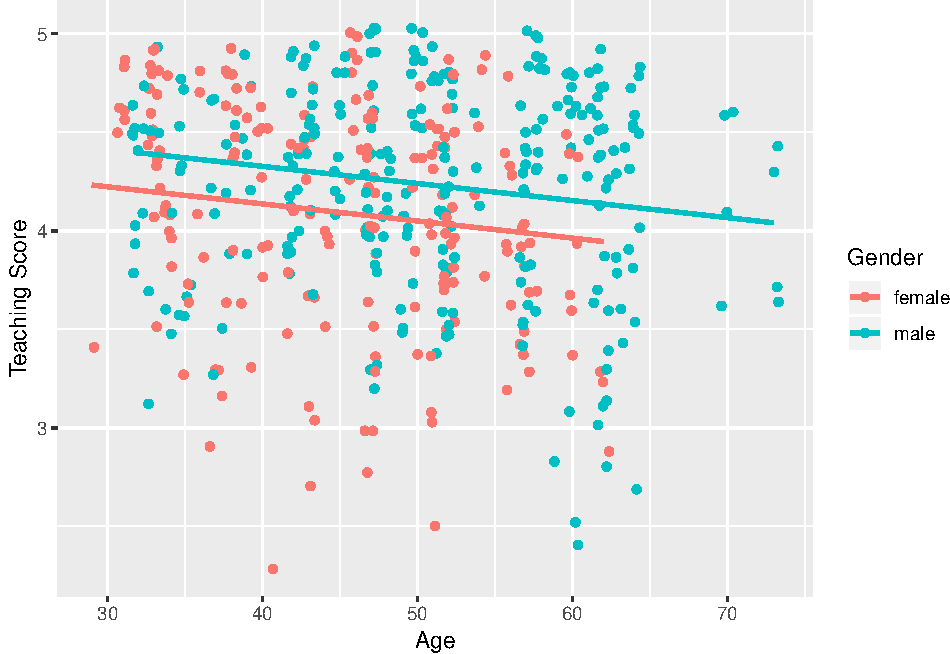
\includegraphics[width=0.85\linewidth]{DAWeek8_files/figure-latex/plot1-1} 

}

\caption{\label{fig:plot1}Model 1: No interaction effect included}\label{fig:plot1}
\end{figure}

\begin{figure}

{\centering 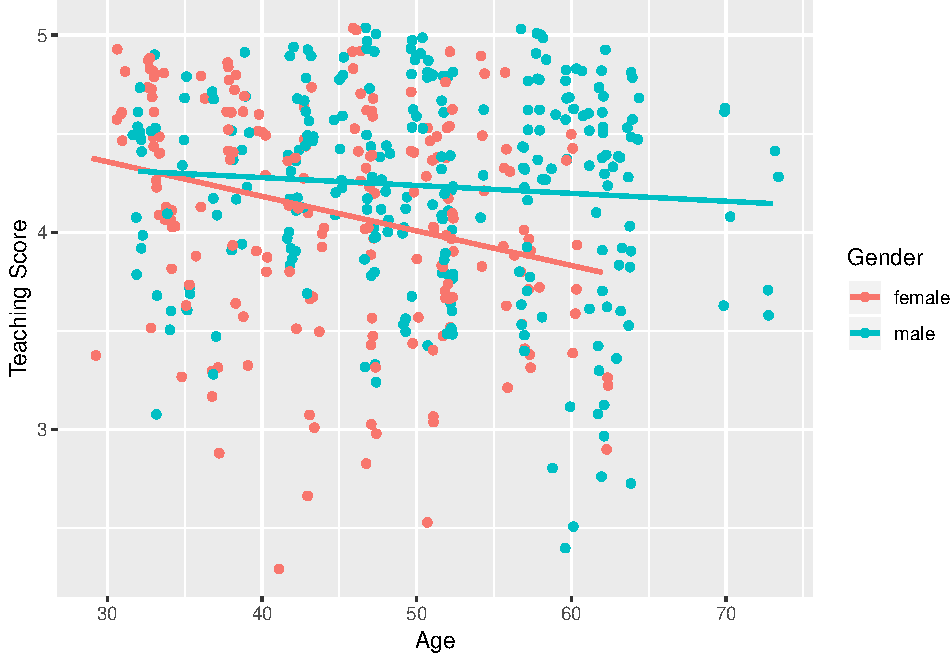
\includegraphics[width=0.85\linewidth]{DAWeek8_files/figure-latex/plot2-1} 

}

\caption{\label{fig:plot2}Model2: Interaction effect included}\label{fig:plot2}
\end{figure}

\newpage  

\textbf{Refresher: Regression Tables}

Let's also recall the regression models we fit. First, the regression
with no interaction effect: note the use of + in the formula.

\begin{longtable}[]{@{}lrrrrrr@{}}
\caption{Model 1: Regression table with no interaction effect
included}\tabularnewline
\toprule
term & estimate & std\_error & statistic & p\_value & lower\_ci &
upper\_ci\tabularnewline
\midrule
\endfirsthead
\toprule
term & estimate & std\_error & statistic & p\_value & lower\_ci &
upper\_ci\tabularnewline
\midrule
\endhead
intercept & 4.484 & 0.125 & 35.792 & 0.000 & 4.238 &
4.730\tabularnewline
age & -0.009 & 0.003 & -3.280 & 0.001 & -0.014 & -0.003\tabularnewline
gendermale & 0.191 & 0.052 & 3.632 & 0.000 & 0.087 &
0.294\tabularnewline
\bottomrule
\end{longtable}

Second, the regression with an interaction effect: note the use of * in
the formula.

\begin{longtable}[]{@{}lrrrrrr@{}}
\caption{Model 2: Regression table with interaction effect
included}\tabularnewline
\toprule
term & estimate & std\_error & statistic & p\_value & lower\_ci &
upper\_ci\tabularnewline
\midrule
\endfirsthead
\toprule
term & estimate & std\_error & statistic & p\_value & lower\_ci &
upper\_ci\tabularnewline
\midrule
\endhead
intercept & 4.883 & 0.205 & 23.795 & 0.000 & 4.480 &
5.286\tabularnewline
age & -0.018 & 0.004 & -3.919 & 0.000 & -0.026 & -0.009\tabularnewline
gendermale & -0.446 & 0.265 & -1.681 & 0.094 & -0.968 &
0.076\tabularnewline
age:gendermale & 0.014 & 0.006 & 2.446 & 0.015 & 0.003 &
0.024\tabularnewline
\bottomrule
\end{longtable}

Notice that, together with the estimated parameter values, the tables
include other information about each estimated parameter in the model,
namely:

\begin{itemize}
\tightlist
\item
  \textbf{std\_error}: the standard error of each parameter estimate
\item
  \textbf{statistic}: the test statistic value used to test the null
  hypothesis that the population parameter is zero
\item
  \textbf{p\_value}: the p-value associated with the test statistic
  under the null hypothesis
\item
  \textbf{lower\_ci} and \textbf{upper\_ci}: the lower and upper bounds
  of the 95\% confidence interval for the population parameter
\end{itemize}

These values are calculated using the theoretical results based on the
standard assumptions that you will have seen in \emph{Regression
Modelling} in first semester. Theses values are \textbf{not} based on
bootstrapping techniques since these become much harder to implement
when working with multiple variables and its beyond the scope of this
course.

\textbf{What is the 95\% Confidence Interval for the difference, on
average, between the (linear) effect age has on the evaluation scores of
male professors and the (linear) effect age has on the evaluation scores
of female professors?}

\begin{itemize}
\tightlist
\item
  \emph{The difference (males - females) between the slopes of the age
  variable is estimated by the age:gendermale term in the interaction
  model. So the linear rate of change in the male evaluation scores is
  likely to be between (0.003, 0.024) higher than the linear rater of
  change in the female evaluation scores}
\end{itemize}

\textbf{By just considering the simpler parallel lines model, what can
we say about the the difference, on average, between the evaluation
scores of male and female professors when age is taken into account?}

\begin{itemize}
\tightlist
\item
  \emph{Its highly likely that, on average, male professors' scores are
  between 0.1 and 0.3 units higher than females professors' scores when
  age is taken into account}
\end{itemize}

\newpage

\section{Inference Using Confidence
Intervals}\label{inference-using-confidence-intervals}

Having described several ways of calculating confidence intervals for
model parameters, we are now in a position to interpret them for the
purposes of statistical inference.

Simple Linear Regression: \(\hat{y}_i = \alpha + \beta x_i\)

Whether we have obtained a confidence interval for \(\beta\) in a simple
linear regression model via bootstrapping or theoretical results based
on assumptions, the interpretation of the interval is the same. As we
saw in Week 7, a confidence interval gives a range of plausible values
for a population parameter.

We can therefore use the confidence interval for \(\beta\) to state a
range of plausible values and, just as usefully, what values are
\textbf{not} plausible. The most common values to compare the confidence
interval of \(\beta\) with is 0 (zero), since \(\beta = 0\) says there
is no (linear) relationship between the outcome variable (\(y\)) and the
explanatory variable (\(x\)). Therefore, if 0 lies within the confidence
interval for \(\beta\) then there is insufficient evidence of a linear
relationship between \(y\) and \(x\). However, if 0 does \textbf{not}
lie within the confidence interval, then we conclude that \(\beta\) is
significantly different from zero and therefore that there is evidence
of a linear relationship between \(y\) and \(x\).

Let's use the confidence interval based on theoretical results for slope
parameter in the SLR model applied to the teacher evaluation
\texttt{score}s with \texttt{age} as the the single explanatory variable
and the instructors' evaluation scores as the outcome variable.

\begin{longtable}[]{@{}lrrrrrr@{}}
\caption{Estimate summaries from the SLR Model of \texttt{score} on
\texttt{age}.}\tabularnewline
\toprule
term & estimate & std\_error & statistic & p\_value & lower\_ci &
upper\_ci\tabularnewline
\midrule
\endfirsthead
\toprule
term & estimate & std\_error & statistic & p\_value & lower\_ci &
upper\_ci\tabularnewline
\midrule
\endhead
intercept & 4.462 & 0.127 & 35.195 & 0.000 & 4.213 &
4.711\tabularnewline
age & -0.006 & 0.003 & -2.311 & 0.021 & -0.011 & -0.001\tabularnewline
\bottomrule
\end{longtable}

\textbf{Based on the fitted SLR model, is there evidence that there is a
statistically significant linear realationship between the age of the
professors and their teaching evaluation score?}

\begin{itemize}
\tightlist
\item
  \emph{Yes - The 95\% CI for the slope parameter is from -0.011 to
  -0.001 which tecnically doesn't contain zero, hence we could conclude
  there is a linear relationship and that for every year the professors
  age the average evaluation score decreases between 0.001 and 0.011
  units. However, clearly the lower bound is so close to zero that we
  would caution that this inference is in fact inconclusive.}
\end{itemize}

\textbf{Multiple Regression}\\
Consider, again, the fitted interaction model for \texttt{score} with
\texttt{age} and \texttt{gender} as the two explanatory variables.

\begin{longtable}[]{@{}lrrrrrr@{}}
\caption{Model 2: Regression table with interaction effect
included}\tabularnewline
\toprule
term & estimate & std\_error & statistic & p\_value & lower\_ci &
upper\_ci\tabularnewline
\midrule
\endfirsthead
\toprule
term & estimate & std\_error & statistic & p\_value & lower\_ci &
upper\_ci\tabularnewline
\midrule
\endhead
intercept & 4.883 & 0.205 & 23.795 & 0.000 & 4.480 &
5.286\tabularnewline
age & -0.018 & 0.004 & -3.919 & 0.000 & -0.026 & -0.009\tabularnewline
gendermale & -0.446 & 0.265 & -1.681 & 0.094 & -0.968 &
0.076\tabularnewline
age:gendermale & 0.014 & 0.006 & 2.446 & 0.015 & 0.003 &
0.024\tabularnewline
\bottomrule
\end{longtable}

\textbf{Based on the fitted interaction model, is there evidence that we
should allow for different rates of change for male and female
professors' teaching scores as they get older?}

\begin{itemize}
\tightlist
\item
  \emph{Yes - The 95\% CI for the interaction term age:gendermale is
  from 0.003 to 0.024 which doesn't contains zero and therefore there is
  evidence of a statistically significant difference in the rate of
  change of the evaluation scores between male and female professors as
  they age. Note that this is a subjective conclusion, since the lower
  bound is close to zero and therefore could be interpretted as
  `inconclusive'.}
\end{itemize}

\newpage

\section{Variable Selection Using Confidence Intervals}\label{sec:CIs}

When there is more than one explanatory variable in a model, the
parameter associated with each explanatory variable is interpreted as
the change in the mean response based on a 1-unit change in the
corresponding explanatory variable \textbf{keeping all other variables
held constant}. Therefore, care must be taken when interpreting the
confidence intervals of each parameter by acknowledging that each are
plausible values \textbf{conditional on all the other explanatory
variables in the model}.

Because of the interdependence between the parameter estimates and the
variables included in the model, choosing which variables to include in
the model is a rather complex task. We will introduce some of the ideas
in the simple case where we have 2 potential explanatory variables
(\(x_1\) and \(x_2\)) and use confidence intervals to decide which
variables will be useful in predicting the outcome variable (\(y\)).

One approach is to consider a hierarchy of models:

\[\hat{y}_i = \alpha + \beta_1 x_{1i} + \beta_2 x_{2i}\]
\[\hat{y}_i = \alpha + \beta_1 x_{1i} ~~~~~~~~~~~~~~~~ \hat{y}_i = \alpha + \beta_2 x_{2i}\]
\[\hat{y}_i = \alpha\]

Within this structure we might take a top-down approach:

\begin{enumerate}
\def\labelenumi{\arabic{enumi}.}
\tightlist
\item
  Fit the most general model, i.e.
  \(\hat{y}_i = \alpha + \beta_1 x_{1i} + \beta_2 x_{2i}\) since we
  believe this is likely to provide a good description of the data.
\item
  Construct confidence intervals for \(\beta_1\) and \(\beta_2\)

  \begin{enumerate}
  \def\labelenumii{\alph{enumii}.}
  \tightlist
  \item
    If both intervals exclude 0 then retain the model with both \(x_1\)
    and \(x_2\).
  \item
    If the interval for \(\beta_1\) contains 0 but that for \(\beta_2\)
    does not, fit the model with \(x_2\) alone.
  \item
    If the interval for \(\beta_2\) contains 0 but that for \(\beta_1\)
    does not, fit the model with \(x_1\) alone.
  \item
    If both intervals include 0 it may still be that a model with one
    variable is useful. In this case the two models with the single
    variables should be fitted and intervals for \(\beta_1\) and
    \(\beta_2\) constructed and compared with 0.
  \end{enumerate}
\end{enumerate}

If we have only a few explanatory variables, then start with the full
model and simplify by removing terms until no further terms can be
removed. When the number of explanatory variables is large the problem
becomes more difficult. We consider this is Section
\ref{sec:comparisons}

Recall that as well as \texttt{age} and \texttt{gender}, there is also a
potential explanatory variable \texttt{bty\_avg} in the \texttt{evals}
data, i.e.~the numerical variable of the average beauty score from a
panel of six students' scores between 1 and 10. We can fit the multiple
regression model with the two continuous explanatory variables
\texttt{age} and \texttt{bty\_avg} as follows:

\begin{Shaded}
\begin{Highlighting}[]
\NormalTok{mlr.model <-}\StringTok{ }\KeywordTok{lm}\NormalTok{(score }\OperatorTok{~}\StringTok{ }\NormalTok{age }\OperatorTok{*}\StringTok{ }\NormalTok{bty_avg, }\DataTypeTok{data =}\NormalTok{ evals)}
\end{Highlighting}
\end{Shaded}

\begin{longtable}[]{@{}lrrrrrr@{}}
\caption{Estimate summaries from the MLR model with age and
bty-avg}\tabularnewline
\toprule
term & estimate & std\_error & statistic & p\_value & lower\_ci &
upper\_ci\tabularnewline
\midrule
\endfirsthead
\toprule
term & estimate & std\_error & statistic & p\_value & lower\_ci &
upper\_ci\tabularnewline
\midrule
\endhead
intercept & 5.156 & 0.368 & 14.019 & 0.000 & 4.433 &
5.879\tabularnewline
age & -0.026 & 0.007 & -3.559 & 0.000 & -0.041 & -0.012\tabularnewline
bty\_avg & -0.188 & 0.076 & -2.480 & 0.013 & -0.337 &
-0.039\tabularnewline
age:bty\_avg & 0.005 & 0.002 & 3.366 & 0.001 & 0.002 &
0.008\tabularnewline
\bottomrule
\end{longtable}

\textbf{Following the process outlined above for choosing which
variables to include in the model, what would be your next step after
fitting this MLR model?}

\begin{itemize}
\tightlist
\item
  \emph{Fit a SLR model with \texttt{bty\_avg} - None of the 95\% CIs
  for the parameters in the model contain zero \textbf{except} that for
  age (-0.008, 0.002), therefore we conclude that \texttt{age} does not
  contribute significantly to the model alongside \texttt{bty\_avg} and
  thus remove it from the model and refit the model with just
  \texttt{bty\_avg}. Note that this is a subjective conclusion, since
  the upper bound is close to zero and therefore could be interpretted
  as `inconclusive'.}
\end{itemize}

\newpage

\section{Model Comparisons Using Objective
Criteria}\label{sec:comparisons}

As noted in Section \ref{sec:CIs}, when the number of potentials
predictor varaibles ilarge the problem of selecting which variables to
include in the final model becomes more difficult. The selection of a
final regression model always involves a compromise:

\begin{itemize}
\tightlist
\item
  Predictive accuracy (improved by including more predictors)
\item
  Parsimony and interpretability (achieved by having less predictors)
\end{itemize}

There are many objective criteria for comparing different models applied
to the same data set. All of them trade off the two objectives above,
i.e.~fit to the data against complexity. Common examples include:

\begin{enumerate}
\def\labelenumi{\arabic{enumi}.}
\tightlist
\item
  The \$R\&2\_\{adj\} values, i.e.~the proportions of total variation of
  response variable explained by the models.
  \[R^2_{adj} = 1 - \frac{RSS/(n-p-1)}{SST/(n-1)} = 100 \times \Bigg[ 1 - \frac{ \sum^n_{i=1} (y_i - \hat{y}_i)^2 / (n-p-1)}{ \sum^n_{i=1} (y_i - \bar{y}_i)^2 / (n-1)} \Bigg]\]

  \begin{itemize}
  \tightlist
  \item
    where

    \begin{itemize}
    \tightlist
    \item
      \(n\) is the sample size
    \item
      \(p\) is the number of parameters in the model
    \item
      \(RSS\) is the residual sum of squares from the fitted model
    \item
      \(SST\) is the total sum of squares around the mean response
    \end{itemize}
  \item
    F ratios and the F-distribution can be used to compare the
    \(R^2_{adj}\) values
  \item
    These can only be used for nested models, i.e.~where one model is a
    particular case of the other
  \end{itemize}
\item
  Akaike's Information Criteria (AIC)
  \[AIC = -2(log-likelihood) + 2p = nlon \Bigg( \frac{RSS}{n} \Bigg) + 2p\]

  \begin{itemize}
  \tightlist
  \item
    A value based on the maximum likelihood function of the parameters
    in the fitted model penalized by the number of parameters in the
    model
  \item
    Can be used to compare any models fitted to the same response
    variable
  \item
    The smaller the AIC the `better' the model, i.e.~no distributional
    results are employed to assess differences
  \end{itemize}
\end{enumerate}

3.Bayesian Information Criteria \[BIC = -2(log-likelihood) + ln(n)p\]

A popular analysis strategy which we shall adopt is to calculate
\(R^2_{adj}\), AIC, and BIC and prefer the models which \emph{minimize}
AIC and BIC and that \textbf{maximize} \(R^2_{adj}\).

To illustrate, let's return to the \texttt{evals} data and the MLR on
the teaching evaluation score \texttt{score} with the two continuous
explanatory variables \texttt{age} and \texttt{bty\_avg} and compare
this with the SLR model with just \texttt{bty\_avg}. To access these
measures for model comparisons we can use the \texttt{glance()} function
in the broom package (not to be confused with the \texttt{glimpse()}
function in the \texttt{dplyr} package).

\begin{Shaded}
\begin{Highlighting}[]
\KeywordTok{library}\NormalTok{(broom)}
\NormalTok{model.comp.values.slr.age <-}\StringTok{ }\KeywordTok{glance}\NormalTok{( }\KeywordTok{lm}\NormalTok{(score }\OperatorTok{~}\StringTok{ }\NormalTok{age, }\DataTypeTok{data =}\NormalTok{ evals) )}
\NormalTok{model.comp.values.slr.age}
\end{Highlighting}
\end{Shaded}

\begin{verbatim}
# A tibble: 1 x 11
  r.squared adj.r.squared sigma statistic p.value    df logLik   AIC   BIC
      <dbl>         <dbl> <dbl>     <dbl>   <dbl> <int>  <dbl> <dbl> <dbl>
1    0.0115       0.00931 0.541      5.34  0.0213     2  -372.  750.  762.
# ... with 2 more variables: deviance <dbl>, df.residual <int>
\end{verbatim}

\begin{Shaded}
\begin{Highlighting}[]
\NormalTok{model.comp.values.slr.bty_avg <-}\StringTok{ }\KeywordTok{glance}\NormalTok{( }\KeywordTok{lm}\NormalTok{(score }\OperatorTok{~}\StringTok{ }\NormalTok{bty_avg, }\DataTypeTok{data =}\NormalTok{ evals) )}
\NormalTok{model.comp.values.slr.bty_avg}
\end{Highlighting}
\end{Shaded}

\begin{verbatim}
# A tibble: 1 x 11
  r.squared adj.r.squared sigma statistic p.value    df logLik   AIC   BIC
      <dbl>         <dbl> <dbl>     <dbl>   <dbl> <int>  <dbl> <dbl> <dbl>
1    0.0350        0.0329 0.535      16.7 5.08e-5     2  -366.  738.  751.
# ... with 2 more variables: deviance <dbl>, df.residual <int>
\end{verbatim}

\begin{Shaded}
\begin{Highlighting}[]
\NormalTok{model.comp.values.mlr <-}\StringTok{ }\KeywordTok{glance}\NormalTok{( }\KeywordTok{lm}\NormalTok{(score }\OperatorTok{~}\StringTok{ }\NormalTok{age }\OperatorTok{+}\StringTok{ }\NormalTok{bty_avg, }\DataTypeTok{data =}\NormalTok{ evals) )}
\NormalTok{model.comp.values.mlr}
\end{Highlighting}
\end{Shaded}

\begin{verbatim}
# A tibble: 1 x 11
  r.squared adj.r.squared sigma statistic p.value    df logLik   AIC   BIC
      <dbl>         <dbl> <dbl>     <dbl>   <dbl> <int>  <dbl> <dbl> <dbl>
1    0.0378        0.0336 0.535      9.03 1.42e-4     3  -366.  739.  756.
# ... with 2 more variables: deviance <dbl>, df.residual <int>
\end{verbatim}

Note that \(R^2_{adj}\), \(AIC\), and \(BIC\) are contained in columns
3, 9, and 10, respectively. To access just these values and combine them
in a single table we use:

\begin{longtable}[]{@{}lrrr@{}}
\caption{Model comparison values for different models}\tabularnewline
\toprule
Model & adj.r.squared & AIC & BIC\tabularnewline
\midrule
\endfirsthead
\toprule
Model & adj.r.squared & AIC & BIC\tabularnewline
\midrule
\endhead
SLR(age) & 0.01 & 749.62 & 762.03\tabularnewline
SLR(bty\_avg) & 0.03 & 738.44 & 750.86\tabularnewline
MLR & 0.03 & 739.12 & 755.67\tabularnewline
\bottomrule
\end{longtable}

\textbf{Based on these values and the model comparison strategy outlined
above, which of these three models would you favor?}

\begin{itemize}
\tightlist
\item
  \emph{The SLR model with \texttt{bty\_avg} - The SLR model with
  \texttt{bty\_avg} has the highest \(R^2_{adj}\) value and the lowest
  \(AIC\) and \(BIC\) values. We note, however, the very low
  \(R^2_{adj}\) values which suggest that none of these models is a good
  fit to the data.}
\end{itemize}

\newpage

\section{A Final Word on Model Selection}\label{sec:Final}

A great deal of care should be taken in selecting predictors for a model
because the values of the regression coefficients depend upon the
variables in the model. Therefore, the predictors included and the order
in which they are entered into the model can have a great impact. In an
ideal world, predictors should be selected based on past research and
new predictors should be added to existing models based on the
theoretical importance of the variables. One thing not to do is select
hundreds of random predictors, bung them all into a regression analysis
and hope for the best.

But in practice there are automatic strategies, such as Stepwise and
Best Subsets regression, based on systematically searching through the
entire list of variables not in the current model to make decisions on
whether each should be included. These strategies need to be handled
with care, and a proper discussion of them is beyond this course. Our
best strategy is a mixture of judgement on what variables should be
included as potential explanatory variables, together with parameter
interval estimation and a comparison of objective measures for assessing
different models. The judgements should be made in the light of advice
from the problem context.

\textbf{Golden Rule for Modelling}

\emph{``The key to modelling data is to only use the objective measures
as a rough guide. In the end the choice of model will involve your own
judgement. You have to be able to defend why you chose a particular
model.''}

\newpage

\section{Further Tasks}\label{sec:Further}

Data was collected on the characteristics of homes in Los Angeles (LA)
in 2010. The data contain the following variables:

\begin{itemize}
\tightlist
\item
  \texttt{city} - the district of LA where the house was located
\item
  \texttt{type} - either SFR (Single Family Residences) or Condo/Twh
  (Condominium/Town House)
\item
  \texttt{bed} - the number of bedrooms
\item
  \texttt{bath} - the number of bathrooms
\item
  \texttt{garage} - the number of car spaces in the garage
\item
  \texttt{sqft} - the floor area of the house (in square feet)
\item
  \texttt{pool} - Y if the house has a pool
\item
  \texttt{spa} - TRUE if the house has a spa
\item
  \texttt{price} - the most recent sales price (US)
\end{itemize}

We are interested in exploring the relationships betwen \texttt{price}
and the other variables.

Read the data into an object called \texttt{LAhomes} and answer the
following questions.

\begin{enumerate}
\def\labelenumi{\alph{enumi}.}
\tightlist
\item
  By looking at the univariate and bivariate distributions on the
  \texttt{price} and \texttt{sqft} variables below, what would be a
  sensible way to proceed if we wanted to model this data? What care
  must be taken if you were to proceed this way?
\end{enumerate}

\includegraphics{DAWeek8_files/figure-latex/unnamed-chunk-8-1.pdf}

\begin{verbatim}
+ *Model the data with count regressing on the `log(price)` and `log(sqft)` including an interaction term `log(price)log(sqft)` because the two covariates are correlated.*  
\end{verbatim}

\begin{enumerate}
\def\labelenumi{\alph{enumi}.}
\setcounter{enumi}{1}
\tightlist
\item
  Fit the simple linear model with \texttt{log(price)} as the response
  and \texttt{log(sqft)} as the predictor. Display the fitted model on a
  scatterplot of the data and construct a bootstrap confidence interval
  (using the percentiles of the bootstrap distribution) for the slope
  parameter in the model and interpret its point and interval estimates.
\end{enumerate}

Hint: Although you can supply the \texttt{lm()} function with terms like
\texttt{log(price)} when you use the \texttt{infer} package to generate
bootstrap intervals you the transformed variable needs to already exist.
Use the \texttt{mutate()} funtion in the \texttt{dplyr} package to
create new transformed variables.

\begin{figure}[H]

{\centering \includegraphics[width=0.85\linewidth]{DAWeek8_files/figure-latex/plot3-1} 

}

\caption{\label{fig:plot3}Model of LA home prices by sqft with interaction inluded}\label{fig:plot3}
\end{figure}

\begin{itemize}
\tightlist
\item
  \emph{The bootstrap CI (using percentiles of the bootstrap
  distribution) for the slope parameter in the model is 1078.26,
  1888.11. For every 1 unit increase in \texttt{sqft} the price of a
  home in LA increases between 1078.26 and 1888.11.}
\end{itemize}

\begin{enumerate}
\def\labelenumi{\alph{enumi}.}
\setcounter{enumi}{2}
\tightlist
\item
  \textbf{Repeat the analysis in part b. but with the log of the number
  of bathrooms (\texttt{bath}) as the single explanatory variable.}
\end{enumerate}

\begin{figure}[H]

{\centering \includegraphics[width=0.85\linewidth]{DAWeek8_files/figure-latex/plot4-1} 

}

\caption{\label{fig:plot4}Model of LA home prices by bath with interaction inluded}\label{fig:plot4}
\end{figure}

\begin{enumerate}
\def\labelenumi{\alph{enumi}.}
\setcounter{enumi}{3}
\tightlist
\item
  **Fit the multiple linear regression model using the log transform of
  all the variables price (as the response) and both sqft and bath (as
  the explanatory variables). Calculate the point and interval estimates
  of the coefficients of the two predictors separately. Compare their
  point and interval estimates to those you calculated in parts b. and
  c. Can you account for the differences?
\end{enumerate}

Hint: Remember that we didn't use bootstrapping to construct the
confidence intervals for parameters in multiple linear regression
models, but rather used the theoretical results based on assumptions.
You can access these estimates using the get\_regression\_table()
function in the moderndive package.**


\end{document}
